\lstdefinelanguage{plaintext}{
  sensitive=false,
  comment=[l]{//},
  morecomment=[s]{/*}{*/},
  identifierstyle=\color{black},
  morestring=[b]',
  morestring=[b]"
}

\lstset
{ 
     language=plaintext,
     basicstyle=\footnotesize,
     numbers=left,
     stepnumber=1,
     showstringspaces=false,
     tabsize=1,
     breaklines=true,
     breakatwhitespace=false,
     frame=leftline
}

\chapter{Analisis}
\label{chap:analisis}
Pada bab ini dijelaskan mengenai analisis aplikasi sejenis, analisis penggunaan JGit dan Selenium WebDriver untuk membangkitkan animasi timelapse, prapengujian, dan analisis fitur aplikasi yang dibangun. 

\section{Analisis Aplikasi Sejenis}
\label{sec:analisis_aplikasi_sejenis}
Saat skripsi ini dibuat, aplikasi sejenis yang digunakan untuk membangkitkan animasi adalah Gource.  
Proyek perangkat lunak ditampilkan oleh Gource sebagai animasi pohon, dimana pusatnya adalah \textit{root directory} dari proyek perangkat lunak\cite{Gource}. Direktori ditampilkan sebagai \textit{branch}, sedangkan \textit{file} ditampilkan sebagai \textit{leaf}. Developer dapat terlihat di \textit{working tree} pada saat mereka berkontribusi untuk proyek.

\begin{figure}[H]
	\centering
		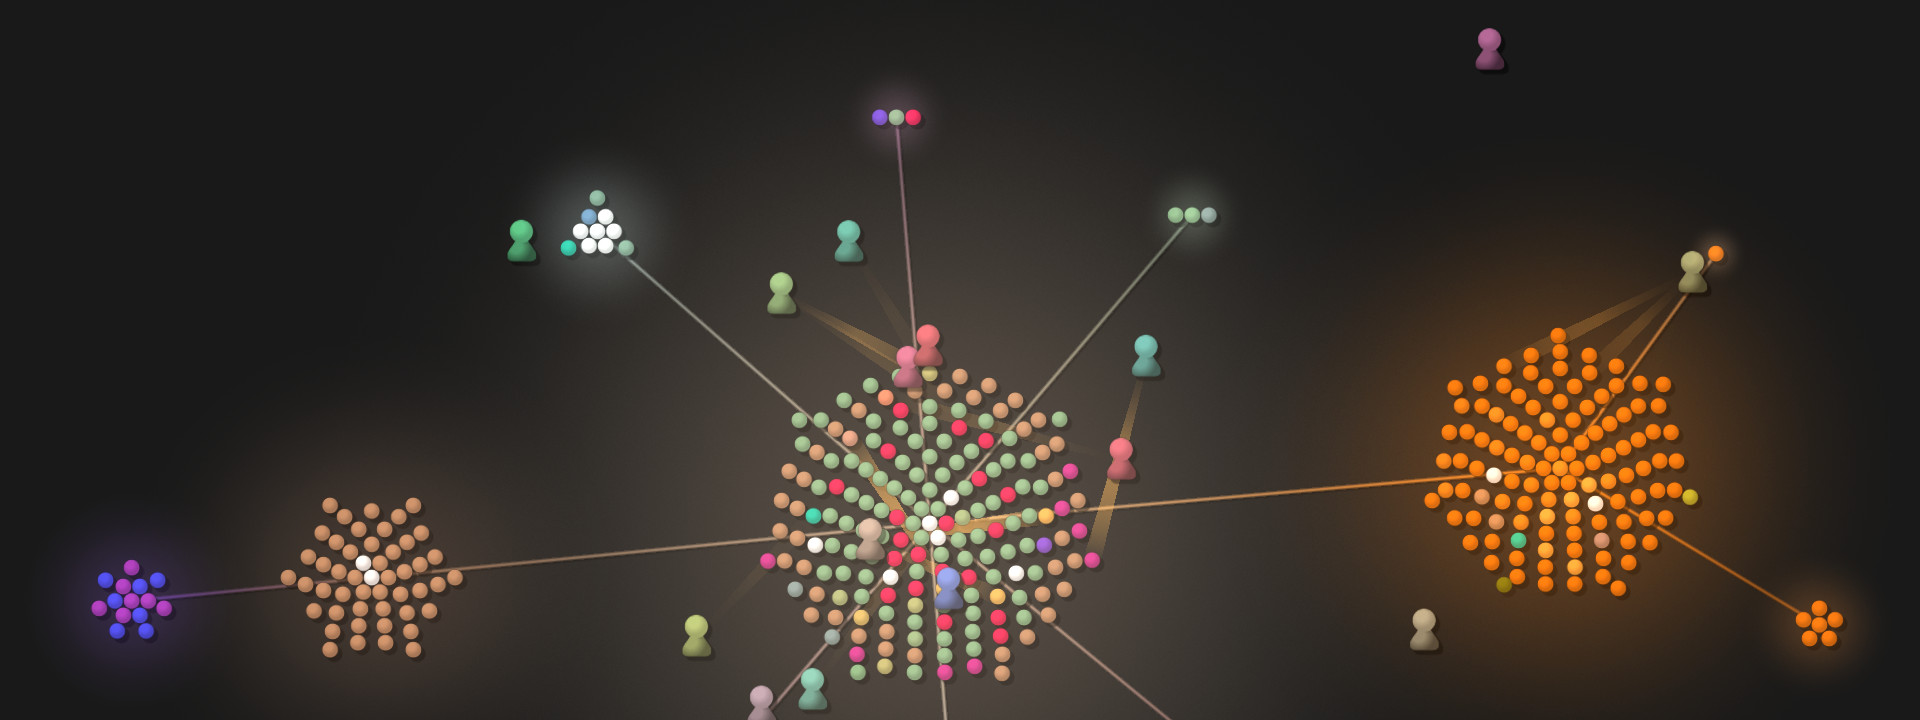
\includegraphics[scale=0.2]{Gambar/gource.jpg}
	\caption{Visualisasi proyek perangkat lunak menggunakan Gource.}
	\label{fig:gource}
\end{figure}

Gambar \ref{fig:gource} menunjukkan contoh visualisasi proyek perangkat lunak menggunakan Gource. Efek cahaya yang terdapat pada Gambar \ref{fig:gource} disebut dengan \textit{bloom}. Pada awalnya ukuran \textit{working tree} tidak terlalu besar. Setiap kali ditambahkan \textit{file} dan \textit{folder} baru, akan dibuat \textit{branch} dan \textit{leaf} baru pada \textit{working tree}.  

\ \\
Gource memiliki beberapa fitur. Fitur-fitur tersebut dapat diatur melalui \textit{command line option}. Berikut ini adalah beberapa \textit{command line option} yang terdapat pada Gource:
\begin{enumerate}
\item \texttt{gource --[WIDTH]x[HEIGHT]}\\
Opsi ini berfungsi untuk mengatur resolusi layar dari animasi. Parameter dari opsi ini adalah lebar dan panjang layar dalam satuan piksel. 

\item \texttt{gource --camera-mode [MODE]}\\
Opsi ini berfungsi untuk mengatur mode kamera pada Gource. Parameter dari opsi ini adalah mode dari kamera. Terdapat dua mode yaitu \textit{overview} dan \textit{track}. Dalam mode \textit{track}, kamera bergerak mengikuti \textit{user} yang sedang aktif. Dalam mode \textit{overview}, kamera menampilkan seluruh repositori.

\item \texttt{gource --path [PATH]}\\
Opsi ini berfungsi untuk mengatur \textit{path} dari direktori yang akan dibuat animasinya. Opsi dari parameter ini adalah \textit{path} dari direktori.

\item \texttt{gource --start-date [YYYY-MM-DD hh:mm:ss +tz] --stop-date [YYYY-MM-DD hh:mm:ss +tz]}\\
Opsi ini berfungsi untuk mengatur periode waktu dalam menampilkan animasi. Parameter dari opsi ini adalah waktu mulai dan waktu akhir dalam format "YYYY-MM-DD hh:mm:ss +tz". Dimana YYYY adalah tahun, MM adalah bulan, DD adalah tanggal, hh adalah jam, mm adalah menit, ss adalah detik, dan +tz adalah zona waktu. Parameter jam, menit, detik, dan zona waktu bersifat opsional.    

\item \texttt{gource --bloom-multiplier [FLOAT] }\\
Opsi ini berfungsi untuk mengatur radius dari efek \textit{bloom}. Parameter dari opsi ini adalah radius dalam format bilangan riil.

\item \texttt{gource --bloom-intensity [FLOAT]}\\
Opsi ini berfungsi untuk mengatur intensitas dari efek \textit{bloom}. Parameter dari opsi ini adalah intensitas \textit{bloom} dalam format bilangan riil.

\item \texttt{gource --disable-bloom}\\
Opsi ini berfungsi untuk menonaktifkan animasi \textit{bloom}.

\item \texttt{gource --date-format [FORMAT]}\\ 
Opsi untuk mengatur format waktu yang ditampilkan pada bagian tengah atas. Opsi dari parameter ini adalah format waktu dalam bentuk \textit{string}.

\item \texttt{gource --background [FFFFFF]}\\
Opsi ini berfungsi untuk mengatur warna \textit{background}. Parameter dari opsi ini adalah warna dalam format heksadesimal.

\item \texttt{gource --background-image [IMAGE]}\\
Opsi ini berfungsi untuk mengatur gambar \textit{background}. Parameter dari opsi ini adalah nama \textit{file} dari gambar.

\item \texttt{gource --font-size [SIZE]}\\
Opsi ini digunakan untuk mengatur ukuran \textit{font} pada tulisan \textit{title} dan tanggal. Parameter dari opsi ini adalah ukuran \textit{font}.  

\item \texttt{gource --font-colour [FFFFFF]}\\
Opsi ini digunakan untuk mengatur warna \textit{font} pada tulisan \textit{title} dan tanggal. Parameter dari opsi ini adalah warna \textit{font} dalam format heksadesimal.

\item \texttt{gource --logo [IMAGE]}\\
Opsi ini berfungsi untuk memasukkan logo. Parameter dari opsi ini adalah nama \textit{file} dari gambar.

\item \texttt{gource --logo-offset [X]x[Y]}\\
Opsi ini berfungsi untuk mengatur posisi dari logo. Parameter dari opsi ini adalah posisi x dan posisi y dari logo. 

\item \texttt{gource --title [TITLE]}\\
Opsi ini berfungsi untuk memberi judul. Dimana judul tersebut ditampilkan pada pojok kiri bawah layar. 

\item \texttt{gource --output-framerate [FPS]}\\
Opsi ini berfungsi untuk mengatur jumlah \textit{frame} per detik pada video animasi. Parameter dari opsi ini adalah jumlah \textit{frame} per detik.

\item \texttt{gource --seconds-per-day [SECONDS]}\\
Opsi ini berfungsi untuk mengatur kecepatan visualisasi. Parameter dari opsi ini adalah waktu yang dibutuhkan untuk menampilkan satu hari.

\item \texttt{gource --hide [DISPLAY-ELEMENT]}\\
Opsi ini berfungsi untuk menyembunyikan satu atau lebih \textit{display element}. Parameter dari opsi ini adalah elemen yang akan disembunyikan. \textit{Display element} yang dapat disembunyikan yaitu:
\begin{itemize}
\item \textit{bloom}: efek \textit{bloom}. 
\item \textit{date}: waktu.  
\item \textit{dirnames}: nama direktori. 
\item \textit{files}: ikon dari berkas. 
\item \textit{filenames}: nama berkas. 
\item \textit{root}: \textit{root directory}.
\item \textit{users}: ikon dari \textit{user}.
\item \textit{usernames}: nama dari \textit{user}.
\end{itemize}
Parameter yang berjumlah lebih dari satu dipisahkan dengan koma, contoh: \textit{bloom},\textit{root},\textit{users}.
\end{enumerate}
 
Gource dapat digunakan untuk berbagai macam proyek perangkat lunak. Program pada skripsi ini hanya akan berfokus untuk proyek perangkat lunak berbasis \textit{web}. Tidak seperti Gource yang menampilkan direktori dan \textit{file} pada animasi, program pada skripsi ini menampilkan \textit{screenshot} dari halaman suatu \textit{website}.      
 
\section{Analisis Penggunaan JGit dan Selenium WebDriver}
\label{sec:analisis_jgit_selenium}
Pada subbab ini dijelaskan mengenai analisis penggunaan JGit dan Selenium WebDriver.

\subsection{Analisis Penggunaan JGit}
\label{subsec:analisis_jgit}
JGit dapat digunakan untuk berinteraksi dengan repositori yang terekam oleh Git. Dimana interaksi ini dapat dilakukan melalui program java. Pada analisis ini dibahas kelas-kelas pada \textit{library} JGit yang digunakan untuk berinteraksi dengan suatu repositori Git. Kelas-kelas yang dipakai yaitu Git, Repository, FileRepository, dan RevCommit.

Untuk dapat berinteraksi dengan suatu repositori Git diperlukan kelas Repository dan Git. Kelas Repository dan FileRepository merepresentasikan suatu repositori Git. Kelas FileRepository merupakan turunan dari kelas Repository. Operasi-operasi pada Git dapat dilakukan dengan menggunakan kelas Git. \textit{Constructor} dari kelas Git menerima parameter bertipe Repository. Repository bersifat abstrak, karena itu tidak bisa diinisialisasi secara langsung. Repository dapat diinisialisasi menggunakan \textit{object} yang bertipe FileRepository. Dimana \textit{constructor} FileRepository menerima parameter berupa alamat dari direktori Git. 

Dibutuhkan beberapa langkah untuk melakukan operasi Git Log. Dari object bertipe Git, dapatkan object bertipe LogCommand dengan memanggil \textit{method} log(). Setelah itu, panggil \textit{method} call() untuk melakukan operasi Git Log. Setelah operasi Git Log dijalankan, akan didapatkan seluruh \textit{commit} pada \textit{branch} yang sedang aktif, dimana seluruh \textit{commit} tersebut berupa \textit{object} yang bertipe Iterable<RevCommit>. Jika histori seperti pada Gambar \ref{fig:DAG} dan saat ini \textit{HEAD} berada di Master, Iterable<RevCommit> akan berisi commit4, commit3, commit2, dan commit1. Jika saat ini \textit{HEAD} berada di BRANCH maka Iterable<RevCommit> akan berisi commit6, commit5, commit2,dan commit1. Operasi Git Log ini nantinya dipakai untuk mendapatkan seluruh histori \textit{commit} dari perangkat lunak berbasis \textit{web}.

\begin{figure}[H]
	\centering
		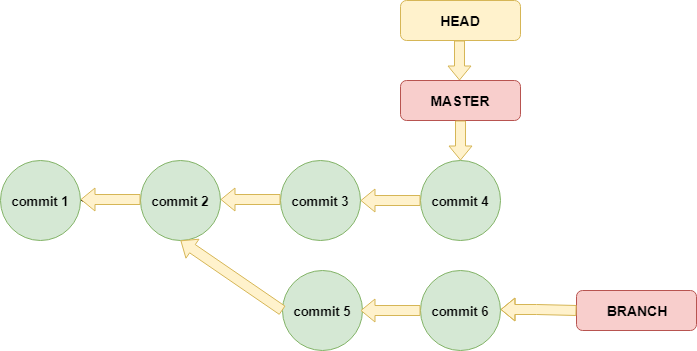
\includegraphics[scale=0.6]{Gambar/DAG.png}
	\caption{Histori \textit{commit} direpresentasikan sebagai Directed Acyclic Graph.}
	\label{fig:DAG}
\end{figure}

Dibutuhkan beberapa langkah untuk melakukan operasi Git Checkout. Dari object bertipe Git, dapatkan object bertipe CheckoutCommand dengan memanggil \textit{method} checkout(). Setelah itu, panggil \textit{method} setName() diikuti dengan parameter berupa \textit{commit ID}. Kemudian panggil \textit{method} call() untuk menjalankan operasi Git Checkout. Setelah opersi Git Checkout dijalankan, \textit{working directory} akan diperbarui sesuai dengan \textit{state} pada \textit{commit} tertentu. Operasi \textit{checkout} ini nantinya akan gigunakan untuk menelusuri \textit{commit} dari perangkat lunak berbasis \textit{web}. Penelusuran ini dilakukan dengan tujuan mendapatkan \textit{screenshot} halaman \textit{web}.    


\subsection{Analisis Penggunaan Selenium WebDriver}
\label{subsec:analisis_selenium}
Selenium WebDriver dapat digunakan untuk mengotomatisasi \textit{web browser}. Pada analisis ini dibahas kelas-kelas pada \textit{library} Selenium WebDriver yang digunakan untuk mengotomatisasi \textit{web browser}. 
Kelas-kelas yang dipakai yaitu WebDriver, ChromeDriver, dan TakesScreenshot.


WebDriver merupakan \textit{interface} utama yang digunakan untuk pengujian. WebDriver dapat diinisialisasi menggunakan \textit{object} dengan tipe ChromeDriver. Setelah melakukan inisialisasi pada WebDriver, \textit{browser} akan dijalankan. Untuk membuka suatu halaman \textit{web}, digunakan \textit{method} get() dengan parameter alamat URL. Gambar \ref{fig:webdriver} menunjukkan Chrome \textit{browser} yang dikontrol oleh ChromeDriver. 

\begin{figure}[H]
	\centering
		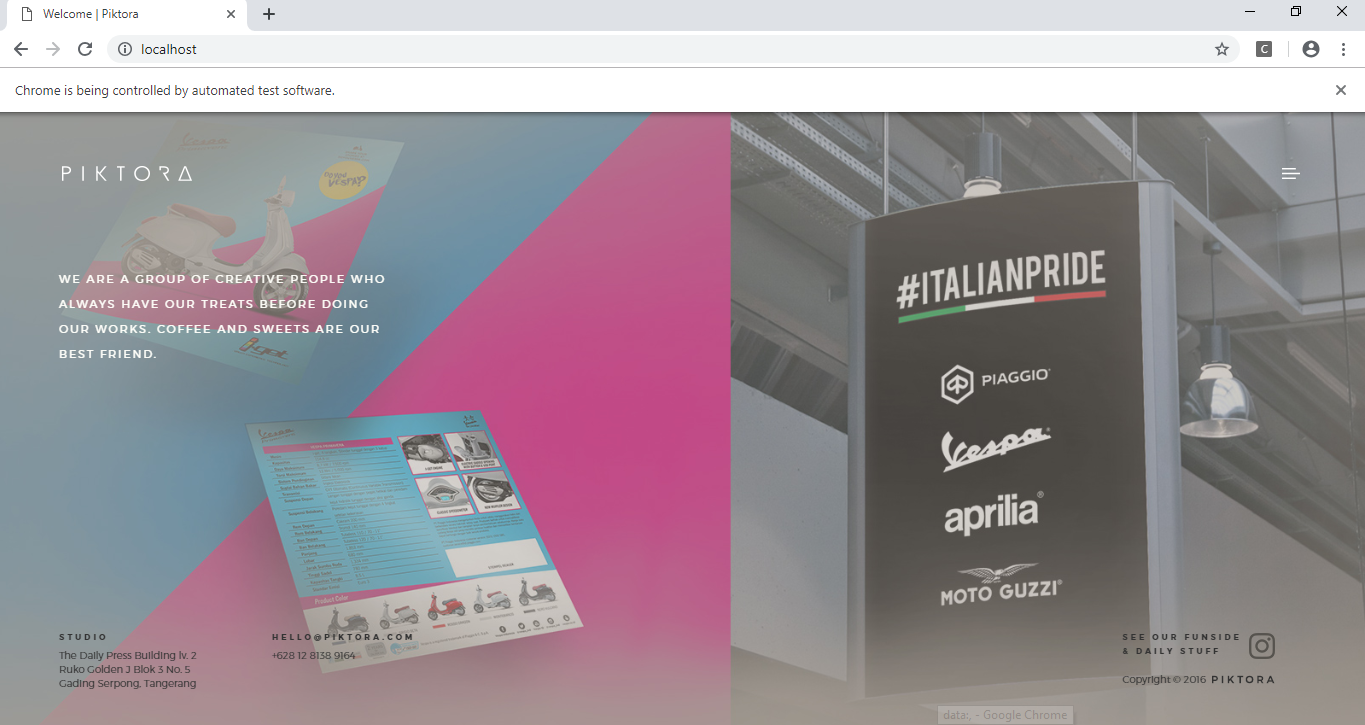
\includegraphics[scale=0.5]{Gambar/ChromeDriver.png}
	\caption{\textit{Browser} yang dikontrol oleh ChromeDriver.}
	\label{fig:webdriver}
\end{figure}


TakesScreenshot merupakan \textit{interface} yang digunakan untuk menangkap \textit{screenshot} halaman \textit{web} pada WebDriver. Kelas ChromeDriver mengimplementasikan \textit{interface} ini. \textit{Method} yang digunakan untuk menangkap \textit{screenshot} adalah getScreenshotAs(), diikuti dengan parameter bertipe OutputType. OutputType ini merupakan \textit{interface} yang digunakan untuk menentukan tipe \textit{output} dari hasil \textit{screenshot}. OutputType yang digunakan pada program dalam skripsi ini adalah File.    



\section{Analisis Fitur Aplikasi yang Dibangun}
\label{sec:analisis_fitur_aplikasi}
Pada skripsi ini, dibuat sebuah perangkat lunak yang dapat membangun animasi \textit{timelapse}
dari pengembangan proyek perangkat lunak berbasis web. Yang akan dibuat animasinya adalah
halaman web dari perangkat lunak. Jumlah halaman berkisar antara satu sampai empat halaman, tergantung pada masukan dari \textit{user}. \textit{Output} dari program adalah \textit{file} hasil animasi yang bertipe GIF. Program dapat menerima masukan dan konfigurasi dari Command Line Option. 

Berikut ini adalah \textit{command line option} yang akan diimplementasikan pada skripsi ini:
\begin{enumerate}
\item \texttt{-project-path [PATH]}\\
Opsi ini berfungsi untuk mengatur \textit{path} dari direktori yang akan dibuat animasinya. Parameter dari opsi ini adalah \textit{path} dari proyek perangkat lunak web yang terekam oleh Git. Opsi ini wajib ada.

\item \texttt{-before-capture [PHP-SCRIPT]}\\
Opsi ini berfungsi untuk menjalankan \textit{script} PHP. \textit{Script} ini dijalankan sebelum melakukan \textit{screenshot}. Parameternya adalah \textit{path} dari \textit{script} PHP. Opsi ini bersifat opsional.

\item \texttt{-capture-url [URL 1, URL 2, URL 3, URL 4]}\\
Opsi ini berfungsi untuk mengatur alamat \textit{url} dari halaman \textit{web}, dimana dilakukan pengambilan \textit{screenshot} pada halaman ini. Jumlah halaman yang dicapture bisa lebih dari satu, dengan jumlah maksimal empat halaman. Parameter dari opsi ini adalah alamat \textit{url} dari halaman \textit{web}, dengan jumlah maksimal empat alamat \textit{url}. Opsi ini wajib ada.

\item \texttt{-seconds-per-commit [SECONDS]}\\
Opsi ini berfungsi untuk mengatur durasi munculnya satu \textit{commit} pada animasi. Parameter dari opsi ini adalah durasi munculnya satu \textit{commit} dalam satuan detik. Parameter harus berupa bilangan bulat atau riil, dimana nilainya lebih besar dari nol. Opsi ini bersifat opsional.

\item \texttt{-title [TITLE]}\\
Opsi ini berfungsi untuk memberi judul. Dimana judul tersebut ditampilkan pada pojok kiri
bawah layar. Opsi ini bersifat opsional. 

\item \texttt{-logo [IMAGE]}\\
Opsi ini berfungsi untuk memasukkan logo. Dimana logo tersebut ditampilkan pada pojok kanan
bawah layar. Parameternya adalah \textit{path} dari \textit{file} gambar. Opsi ini bersifat opsional.

\item \texttt{-start-commit [ID] -stop-commit [ID]}\\
Opsi ini berfungsi untuk mengatur rentang \textit{commit} yang akan dibuat animasinya. Parameter dari opsi ini adalah \textit{commit ID} awal dan \textit{commit ID} akhir, dimana panjang \textit{commit ID} adalah tujuh karakter. Opsi ini bersifat opsional. 
\end{enumerate}

\ \\
Opsi \texttt{-path}, \texttt{-title}, dan \texttt{-image} mengacu pada opsi yang terdapat pada Gource. Opsi \texttt{-start-commit -stop-commit} dan \texttt{-seconds-per-commit} mengacu pada Gource, dengan sedikit penyesuaian.  Opsi \texttt{--seconds-per-day} pada Gource menyatakan durasi munculnya satu hari, sedangkan Opsi \texttt{-seconds-per-commit} menyatakan durasi munculnya satu \textit{commit}. Opsi \texttt{--start-date --stop-date} pada Gource dan opsi \texttt{-start-commit -stop-commit} mengatur periode dalam menampilkan animasi. Pada Gource, periode yang digunakan adalah rentang waktu berupa tanggal, bulan, dan tahun. Sedangkan pada opsi \texttt{-start-commit -stop-commit}, rentangnya berupa \textit{commit} ID. Opsi \texttt{-before-capture} dan \texttt{-capture-url} tidak mengacu pada Gource. Kedua opsi tersebut secara khusus dibuat karena program pada skripsi ini membuat animasi \textit{timelapse} dari kumpulan halaman \textit{web}, sedangkan program Gource membuat animasi dari struktur \textit{folder} atau \textit{file}.           
  
 
Program pada skripsi ini memiliki satu fitur. Fitur tersebut adalah membangkitkan animasi \textit{timelapse}.
Penjelasan fitur dapat dilihat pada Gambar \ref{fig:uc} dan Tabel \ref{tab:tabel_sc_animasi}.


\begin{figure}[H]
	\centering
		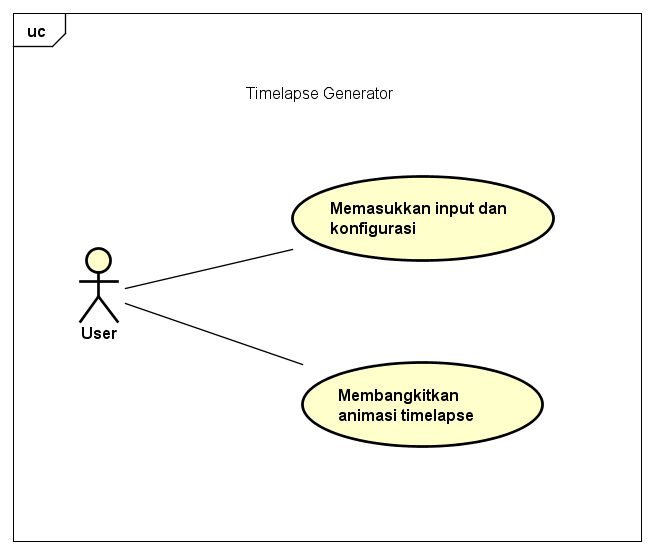
\includegraphics[scale=0.8]{Gambar/UseCaseDiagram1.png}
	\caption{\textit{Use case diagram} perangkat lunak.}
	\label{fig:uc}
\end{figure}
\begin{table}[]
    \centering
    \begin{tabular}{|p{3cm}|p{10cm}|}
    \hline
        Nama & Membangkitkan animasi \textit{timelapse}\\
    \hline
    \hline
        Deskripsi & Fitur untuk membangkitkan animasi timelapse dari pengembangan proyek perangkat lunak berbasis web\\
    \hline
        Aktor & \textit{User} \\
    \hline
        Pos-kondisi &  File animasi bertipe GIF berhasil dibuat\\
    \hline
        Skenario & 
        \begin{enumerate}
        \item Sistem membaca masukan \textit{input} dari Command Line Option.
            \item Sistem menelusuri histori perkembangan perangkat lunak berbasis \textit{web} dengan fitur
Git. Saat menelusuri histori perkembangan perangkat lunak, sistem mengambil \textit{screenshot} dari halaman web menggunakan SeleniumWebDriver.
            \item Sistem menggabungkan file \textit{screenshot} menjadi satu file bertipe GIF.
        \end{enumerate}\\
    \hline
    \end{tabular}
    \caption{\textit{Scenario case} membangkitkan animasi \textit{timelapse}}
    \label{tab:tabel_sc_animasi}
\end{table}


%\subsection{Langkah-Langkah dalam Membangkitkan Animasi Timelapse}
%\label{subsec:langkah_animasi}
%Setelah melakukan analisis pada subbab \ref{subsec:analisis_jgit} sampai subbab \ref{subsec:analisis_selenium}, dapat dibuat langkah-langkah untuk membangkitkan animasi \textit{timelapse}. 
\ \\

Langkah-langkah untuk membangkitkan animasi \textit{timelapse} adalah sebagai berikut:\\
\begin{enumerate}
\item Program membaca argumen Command Line menggunakan Apache Commons CLI.
\item Program mendapatkan seluruh \textit{commit} histori dari proyek perangkat lunak berbasis web menggunakan JGit.
\item Program membuka semua \textit{browser} menggunakan Selenium WebDriver. Jumlah \textit{browser} bergantung pada jumlah argumen dari Option \texttt{-capture-url}.
\item Program melakukan \textit{checkout} dalam suatu rentang \textit{commit} tertentu. Jika tidak terdapat Option \texttt{-start-commit} dan Option \texttt{-stop-commit}, akan dilakukan \textit{checkout} ke semua \textit{commit}.
\item Program melakukan \textit{checkout} ke suatu \textit{commit}. 
\item Program menjalankan \textit{script} PHP jika terdapat Option \texttt{-before-capture}.
\item Program membuka setiap URL yang didapatkan dari Option \texttt{-capture-url} menggunakan Selenium WebDriver. Setiap \textit{browser} membuka URL yang berbeda.
\item Selenium WebDriver kemudian mengambil \textit{screenshot} pada semua \textit{browser}.
\item Jika saat ini sedang berada pada \textit{commit} terakhir, lanjut ke langkah berikutnya. Jika tidak, ulangi langkah 5-8 untuk \textit{commit} selanjutnya.
\item Jika terdapat lebih dari satu \textit{browser}, hasil \textit{screenshot} dari setiap \textit{browser} digabungkan menjadi satu gambar baru. 
\item Program menambahkan judul di pojok kiri bawah jika terdapat Option \texttt{-title}.
\item Program menambahkan logo di pojok kanan bawah jika terdapat Option \texttt{-logo}.  
\item Menggabungkan semua \textit{file} gambar menjadi satu \textit{file} bertipe GIF.
\end{enumerate}

Penulis menggunakan \textit{library} yang didapatkan dari internet\footnote{http://elliot.kroo.net/software/java/GifSequenceWriter} untuk menggabungkan gambar menjadi \textit{file} GIF.


\section{Prapengujian Website Piktora}
\label{sec:prapengujian}
Pengujian dilakukan dengan proyek Piktora sebagai input dari program. Piktora\footnote{http://www.piktora.com} merupakan situs \textit{web} yang menawarkan layanan  \textit{creative design} dan \textit{branding}. Layanan yang ditawarkan berupa \textit{graphic design} untuk poster, \textit{banner}, \textit{website}, dan aplikasi \textit{mobile}. Repositori dari situs \textit{web} ini disimpan pada Gitlab\footnote{https://gitlab.com/PNDevworks/Piktora}, dibutuhkan akses khusus untuk membuka repositori tersebut. Piktora dibangun dengan php  menggunakan framework Code Igniter. Piktora menggunakan MySQL sebagai basis datanya. 

Prapengujian ini hanya menggunakan dua parameter, yaitu project-path dan capture-url(lihat subbab \ref{sec:analisis_fitur_aplikasi}). Pengujian dilakukan menggunakan prototipe program yg akan dilengkapi pada Bab \ref{chap:implementasidanpengujian}. Berikut adalah spesifikasi perangkat keras dan perangkat lunak yang digunakan untuk prapengujian:
\begin{itemize}
\item Processor: Intel Core i3 4030U
\item RAM: 6GB
\item Sistem Operasi: Windows 10 pro 64-bit
\item Versi Apache HTTP Server: 2.4.29
\item Versi MySQL Server: 5.5.5
\item Versi Netbeans: 8.1
\item Versi Google Chrome: 73.0.3683.86
\end{itemize}
Apache HTTP Server digunakan sebagai \textit{web server} lokal. MySQL Server digunakan untuk menyimpan basis data secara lokal dan juga digunakan sebagai \textit{database server} lokal. 

%\begin{enumerate}
%\item Program mengambil input dari parameter menggunakan Apache Commons CLI.
%\item Program mendapatkan seluruh \textit{commit} histori dari proyek Piktora menggunakan JGit.
%\item Program melakukan \textit{checkout} ke \textit{commit} pertama.
%\item Program menjalankan halaman proyek Piktora di \textit{localhost} menggunakan SeleniumWebDriver.
%\item Selenium WebDriver kemudian mengambil \textit{screenshot} pada halaman \textit{web} Piktora.
%\item Langkah 3-5 diulangi untuk seluruh \textit{commit}.
%\item Menggabungkan semua \textit{file} gambar menjadi satu \textit{file} bertipe GIF.
%\end{enumerate}
%\ \\

Pada proyek Piktora terdapat 58 \textit{commit}. Listing \ref{lst:all_commit_piktora} menunjukkan histori \textit{commit} pada proyek Piktora, histori didapatkan dengan menjalankan operasi Git Log pada terminal. Setelah dilakukan pengujian terdapat beberapa masalah. Masalah tersebut yaitu perbedaan letak \textit{file}, migrasi \textit{database}, dan konfigurasi \textit{database}. Masalah-masalah tersebut dibahas pada subbab \ref{subsec:perbedaan_letak_file} sampai \ref{subsec:migrasi_database}.

\begin{lstlisting}[caption={Histori \textit{commit} pada proyek Piktora},label={lst:all_commit_piktora},language=plaintext]
315d374 -  Oct 31 16:52:46 2016 :  Basic CI files + htaccess & webconfig + database.php ignore

27ce3d4 -  Nov 5 13:12:43 2016 :  setup environment for piktora
65f0c9c -  Nov 5 19:22:58 2016 :  * create structure for all pages * add dummy images

bffbae1 -  Nov 8 18:00:32 2016 :  - basic structure (navbar semi complete) - add fonts

5c59916 -  Nov 8 19:51:18 2016 :  implement navbar, footer, and projects/ page
7738380 -  Nov 8 20:05:27 2016 :  fix pc and ipad navbar fontsize
26bdbee -  Nov 8 20:16:33 2016 :  fix position image for desktop /projects
3db3ce8 -  Nov 9 00:28:27 2016 :  - implements project details page - fix some minor issue - add some project image

5ef34fa -  Nov 13 13:01:06 2016 :  implement about us (raw version)
3caf535 -  Nov 15 11:55:15 2016 :  fix minor issues view/about: - background-image position. Make it to the center position - slick.js img need to set to inline

c5eb3b6 -  Nov 15 13:02:42 2016 :  implement /welcome page
ade9216 -  Nov 15 13:12:08 2016 :  fix minor issues: - move style footer to global - add space before PIKTORA

c77b5b3 -  Nov 18 18:18:25 2016 :  implement /contact
b42b819 -  Nov 18 21:22:22 2016 :  cange a href to style cursor: pointer
3eb7af8 -  Nov 21 16:09:40 2016 :  .htaccess to be compatible with cloud kilat
e87e84b -  Nov 22 14:53:45 2016 :  - change vw to 100% - add captcha
ff8d829 -  Nov 22 15:22:53 2016 :  Solved captcha font load: use otf instead of ttf Also: create directory assets/img/captcha and ignore everything inside

dc87342 -  Nov 22 15:49:03 2016 :  - implement captcha code - remove wrong css
9ebe433 -  Nov 22 16:12:44 2016 :  add scroll feature in project/
f0f7270 -  Nov 23 15:17:42 2016 :  Added Google PHP Client v2 See https://github.com/google/google-api-php-client

57a239b -  Nov 23 15:19:57 2016 :  Merge origin/master
e2dfebe -  Nov 27 14:42:24 2016 :  - remove blue outline when click with slick - change background image in about to newest one

a19e7f2 -  Nov 27 15:24:42 2016 :  Detailing dari Edina: 1. Hal. Project Detail, font coba diperkecil saja mungkin ya. 3. Beberapa ukuran font dan spacing ada yang kurang pas sedikit, terlampir detail revisinya ya (file pdf) 4. Footer dibuat selalu stay terus di bagian bawah dengan posisi yang selalu sama. Di home & contact sudah sama, namun di hal. product posisinya agak lebih naik.

3d79d0a - Nov 27 15:29:58 2016 : fix minor issue
0fcd958 - Nov 28 10:11:06 2016 : add raw admin contents
add3974 - Nov 28 12:03:21 2016 : add summernote, implement read project
0680488 - Nov 29 12:38:23 2016 : update admin for projects
fbe7639 - Nov 29 13:10:30 2016 : implement admin for home
db0cedd - Nov 29 13:38:29 2016 : - implementasi database bagian user - upload 9 gambar contoh project

0fe9aaf - Nov 29 14:17:20 2016 : ubah warna garis captcha
f2326dd - Nov 29 14:44:51 2016 : - lewati proses otentikasi sementara
f78cdb4 - Dec 2 12:10:47 2016 : (trying to) fix issue #2
ef9b62b - Dec 2 17:09:58 2016 : revisi dari edina ke-2
c689aa8 - Dec 2 17:11:13 2016 : perbaikan admin sedikit
c4e9576 - Dec 2 17:14:06 2016 : perbaikan di /contact, kelewat
02d04f1 - Dec 5 14:55:20 2016 : tambah wording
a4e4858 - Dec 5 15:08:59 2016 : perbaikan kata2 sedikit
bbd82c2 - Dec 6 10:41:40 2016 : implementasi email
f8c64fc - Dec 6 11:03:08 2016 : change to httpdocs
eb49c2b - Dec 6 11:35:20 2016 : hapus migrasi script di admin
ace1988 - Dec 6 11:39:00 2016 : change overflow to auto
627e65b - Dec 6 11:45:26 2016 : modify database back to local
0896f81 - Dec 7 16:08:30 2016 : update home versi mobile jadi baru (revisi dari Edina)

5cf1292 - Dec 7 16:21:01 2016 : ubah background di about menjadi tidak pecah
c83f4aa - Thu Dec 15 15:04:30 2016 : remove piktora secrets
57f5ea4 - Thu Dec 15 15:09:43 2016 : remove unimportant data
7931c21 - Dec 24 18:40:41 2016 : edit wording
9b0a302 - Dec 25 06:03:50 2016 : Another wording fix
f1ea410 - Thu Jan 5 15:23:32 2017 : fix instagram link
1880a88 - Thu Jan 5 15:24:12 2017 : Merge branch 'master' of https://github.com/pascalalfadian/Piktora

286aa78 - Jan 16 12:48:45 2017 : Perbaikan wording di admin edit project
33702c2 - Feb 21 13:31:08 2017 : change email sender to piktora@mailgun.dnartworks.com.au

18c39ef - Thu Apr 13 15:21:49 2017 : Test commit (in gitlab). Nothing much important
9bfde3c - Apr 17 15:09:54 2017 : add ignore sftp-config.json
38711f0 - Apr 17 15:15:03 2017 : fix bug ugly display when projects too high
9f041ef - May 15 10:40:16 2017 : set insta url to https://www.instagram.com/piktorastudio/

6a085c1 - Dec 12 14:38:38 2017 : Update company address
89000be - Jan 12 12:25:30 2018 : Update new company address
\end{lstlisting}


\subsection{Perbedaan Letak \textit{File}}
\label{subsec:perbedaan_letak_file}
Pada \textit{commit} 315d374(31 Oktober 2016) s.d. bbd82c2(6 Desember 2016) halaman \textit{web} proyek Piktora tidak bisa dibuka. Hal ini disebabkan oleh perbedaan letak \textit{file} "index.php". Pada \textit{commit} 315d374(31 Oktober 2016) s.d. bbd82c2(6 Desember 2016), \textit{file} "index.php" berada pada \textit{folder} "www", sedangkan pada \textit{commit} f8c64fc(6 Desember 2016) s.d. 89000be(12 Januari 2018) \textit{file} "index.php" berada pada \textit{folder} "httpdocs". Akibat adanya perbedaan letak \textit{file} tersebut, maka
konfigurasi dari apache harus diubah.


Solusi untuk mengatasi masalah ini adalah dengan menambahkan \textit{command line option} yang menerima sebuah \textit{script} PHP. \textit{Script} PHP ini akan mengecek letak \textit{file} "index.php" pada \textit{folder} "www" dan "httpdocs". \textit{Script} kemudian akan mengecek \textit{directory root} apache pada \textit{file} "httpd.conf".  Jika \textit{directory root} sudah mengarah ke \textit{folder} tempat "index.php" berada, maka \textit{script} tidak akan mengubah isi \textit{file} "httpd.conf". Jika \textit{directory root} tidak mengarah ke \textit{folder} tempat "index.php" berada, maka \textit{script} akan mengubah \textit{directory root} pada \textit{file} "httpd.conf" dan melakukan \textit{restart} pada apache. \textit{Script} PHP ini akan dijalankan sebelum melakukan migrasi \textit{database}.   


\subsection{Permasalahan Konfigurasi \textit{Database}}
\label{subsec:konfigurasi_database}
Pada \textit{commit} f8c64fc(6 Desember 2016) s.d. ace1988(6 Desember 2016), halaman \textit{web} tidak bisa dibuka. Hal ini disebabkan karena perbedaan konfigurasi pada \textit{file} "database.php". Pada \textit{commit} f8c64fc(6 Desember 2016) s.d. 57f5ea4(15 Desember 2016) dan \textit{commit} f1ea410(5 Januari 2017), di dalam \textit{file} "database.php" terdapat \textit{password} . \textit{Commit} lainnya tidak terdapat \textit{password} pada \textit{file} "database.php". Penulis menggunakan \textit{password} \texttt{"piktora"} pada konfigurasi \textit{database} di MySQL Server.

\begin{lstlisting}[caption={Isi \textit{file} "database.php" pada \textit{commit} f8c64fc(6 Desember 2016)},label={lst:piktora_commit_f8c64fc},language=plaintext]
$active_group = 'default';
$query_builder = TRUE;

$db['default'] = array(
	'dsn'	=> '',
	'hostname' => 'localhost',
	'username' => 'piktora',
	'password' => 'dmHx64%6',
	'database' => 'piktora',
	'dbdriver' => 'mysqli',
	'dbprefix' => '',
	'pconnect' => FALSE,
	'db_debug' => (ENVIRONMENT !== 'production'),
	'cache_on' => FALSE,
	'cachedir' => '',
	'char_set' => 'utf8',
	'dbcollat' => 'utf8_general_ci',
	'swap_pre' => '',
	'encrypt' => FALSE,
	'compress' => FALSE,
	'stricton' => FALSE,
	'failover' => array(),
	'save_queries' => TRUE
);
\end{lstlisting}

Listing \ref{lst:piktora_commit_f8c64fc} merupakan isi dari \textit{file} "database.php" pada \textit{commit} f8c64fc(6 Desember 2016). Dapat dilihat bahwa \textit{password} yang terdapat pada \textit{file} "database.php" adalah \texttt{dmHx64\%6}. \textit{Commit} f8c64fc(6 Desember 2016) s.d. ace1988(6 Desember 2016) menggunakan \textit{password} \texttt{dmHx64\%6}, sedangkan \textit{commit} 627e65b(6 Desember 2016) s.d. 57f5ea4(15 Desember 2016) dan f1ea410(5 Januari 2017) menggunakan \textit{password} \texttt{piktora}. Karena konfigurasi \textit{password} pada \textit{file} "database.php" dan phpMyAdmin berbeda, halaman \textit{website} pada \textit{commit} f8c64fc(6 Desember 2016) s.d. ace1988(6 Desember 2016) tidak bisa dibuka. 

Sama seperti subbab \ref{subsec:perbedaan_letak_file}, solusi untuk mengatasi masalah ini adalah dengan menambahkan \textit{command line option} yang menerima sebuah \textit{script} PHP. \textit{Script} ini akan mengecek \textit{password} yang terdapat pada \textit{file} "database.php". Jika tidak ditemukan \textit{password} atau ditemukan \textit{password} berupa \texttt{piktora}, maka \textit{script} tidak akan mengubah isi \textit{file} "database.php". Jika ditemukan \textit{password} berupa \texttt{dmHx64\%6}, maka \textit{script} akan mengubah \textit{password} menjadi \texttt{piktora}. 

\subsection{Permasalahan Migrasi \textit{Database}}
\label{subsec:migrasi_database}

Pada \textit{commit} 3d79d0a(27 Nov 2016), terjadi \textit{error} saat melakukan migrasi database. Pada \textit{commit} a19e7f2(27 November 2016), terdapat satu \textit{file} untuk melakukan migrasi yaitu "20161122150000\_Structure.php". Pada \textit{commit} 3d79d0a(27 Nov 2016) terdapat dua \textit{file} untuk melakukan migrasi yaitu "20161122150000\_Structure.php" dan "20161122150001\_InitialData.php". Pada \textit{commit} a19e7f2(27 November 2016) \textit{file} "20161122150001\_InitialData.php" dijalankan saat melakukan migrasi. Versi migrasi \textit{database} menjadi "20161122150000". Pada \textit{commit} 3d79d0a(27 Nov 2016), \textit{file} "20161122150000\_Structure.php" tidak dijalankan karena dianggap sama dengan versi migrasi \textit{database} saat ini. Hanya \textit{file} "20161122150001\_InitialData.php" yang dijalankan pada \textit{commit} 3d79d0a(27 Nov 2016). Isi \textit{file} "20161122150001\_InitialData.php" pada \textit{commit} a19e7f2(27 November 2016) dan 3d79d0a(27 Nov 2016) berbeda. Hal ini yang menyebabkan terjadinya \textit{error} saat melakukan migrasi database.  

Sama seperti subbab \ref{subsec:perbedaan_letak_file}, solusi untuk mengatasi masalah ini adalah dengan menambahkan \textit{command line option} yang menerima sebuah \textit{script} PHP. \textit{Script} ini akan melakukan dua pekerjaan. Pertama, \textit{script} akan menghapus \textit{database} piktora. Setelah itu \textit{script} akan membuat \textit{database} piktora. \textit{Script} akan dijalankan sebelum melakukan migrasi \textit{database}. 
 


